\subsubsection{\stid{6.01} LANL ATDM Data and Visualization} 

\paragraph{Overview} 
The LANL ATDM Data and Visualization project develops scalable
systems software for the generation, analysis, and management of data
produced by ECP applications. This project is essential for ECP because
existing systems software is inadequate with respect to deploying advanced
data collection and analysis capabilities into HPC data centers. Existing
software cannot leverage the enormous performance and data capacity
provided within Exascale data centers such that scientists can effectively
generate insight using the data generated by extreme scale
simulations.

Scientific simulations running on Exascale platforms will
continue to have access to enormous solid-state storage tiers that provide 
opportunities for rapid data acquisition. Massive campaign storage
systems built from affordable media offer the opportunity for maintaining
large data sets over longer time periods to support longer duration
simulations and accompanying analysis. Finally, advanced monitoring frameworks
built using time-series databases and analysis storage systems are deploying
within HPC data centers. Each of these systems requires significant systems
software development and integration efforts to create new opportunities for data
management within scientific applications, analysis codes, and HPC
facilities. Upon completion of our project, domain scientists will
leverage these new capabilities to improve the
time to insight for scientists using extreme scale scientific simulations.

\paragraph{Key  Challenges}
%\textit{Describe what is hard to do, why it is challenging.}
Re-architecting storage systems to impact both applications and facilities is
challenging both in its breadth and depth. Fundamentally, our approach is
focused on unlocking the value that currently exists within scientific data,
but has traditionally been too time consuming to extract. As part of these
efforts we've identified the need for software and facility infrastructure
that supports finding data within the diverse set of storage resources.
Similarly, our efforts to better provide in-application support for modern
analysis techniques require careful attention to performance, memory use, and
data reduction without loss of insight. 

\paragraph{Solution Strategy}
%\textit{Describe your basic strategy for addressing the challenges.}
The LANL ATDM Data and Visualization ECP project is focused on delivering new
systems software capabilities for creating, analyzing, and managing data for
Exascale scientific applications and Exascale data centers. We have identified
4 distinct areas that are in need of specific improvements.

MarFS is the only campaign storage system within the DOE complex and is
also the only HPC storage system built using scale-out principles with affordable
SMR hard drives. The LANL monitoring stack is leveraging available open source
software to build dashboards for monitoring both the data center and
scientific application performance. Finally, the application level software
technologies, Cinema and HXHIM, are being developed in coordination with
LANL's ECP application NGC to ensure that data collected during the simulation
execution is of appropriate frequency, resolution, and viewport for later
analysis and visualization by scientists. Cinema is an innovative way of
capturing, storing and exploring extreme scale scientific data. Cinema is
essential for ECP because it embodies approaches to maximize insight from
extreme-scale simulation results while minimizing data footprint 

\paragraph{Recent Progress}
%\textit{Describe what you have done recently.  It would be good to have some
%kind of figure or diagram in this section.}
The MarFS file system is currently deployed as the campaign storage tier
with over 60PB of capacity currently under management in our secure computing
environment. Recent progress includes the development of a new highly
resilient backend based on nested parity. We have also extended our top-level
erasure approach to use RDMA operations for more efficient coding and data movement.

The LANL monitoring stack has been successfully deployed into multiple
computing enclaves within LANL's HPC facility, including LANL's secure
computing environment. Our approach currently supports data ingest and
analysis by system administrators, data analysts, and code teams with multiple
dashboards for each role. We continue to refine our security approach to
ensure that new monitoring monitoring dashboards comply with the requirements
of LANL's CCB, the voting body for ensuring that all LANL deployments are
secured appropriately. The use of our monitoring system by application teams
(which monitor information that includes classified data) has required a
highly granular approach to storage and access roles -- but also makes it more
broadly useful and provides direct benefit to the code teams and users.

\begin{figure}[htb]
	\centering
	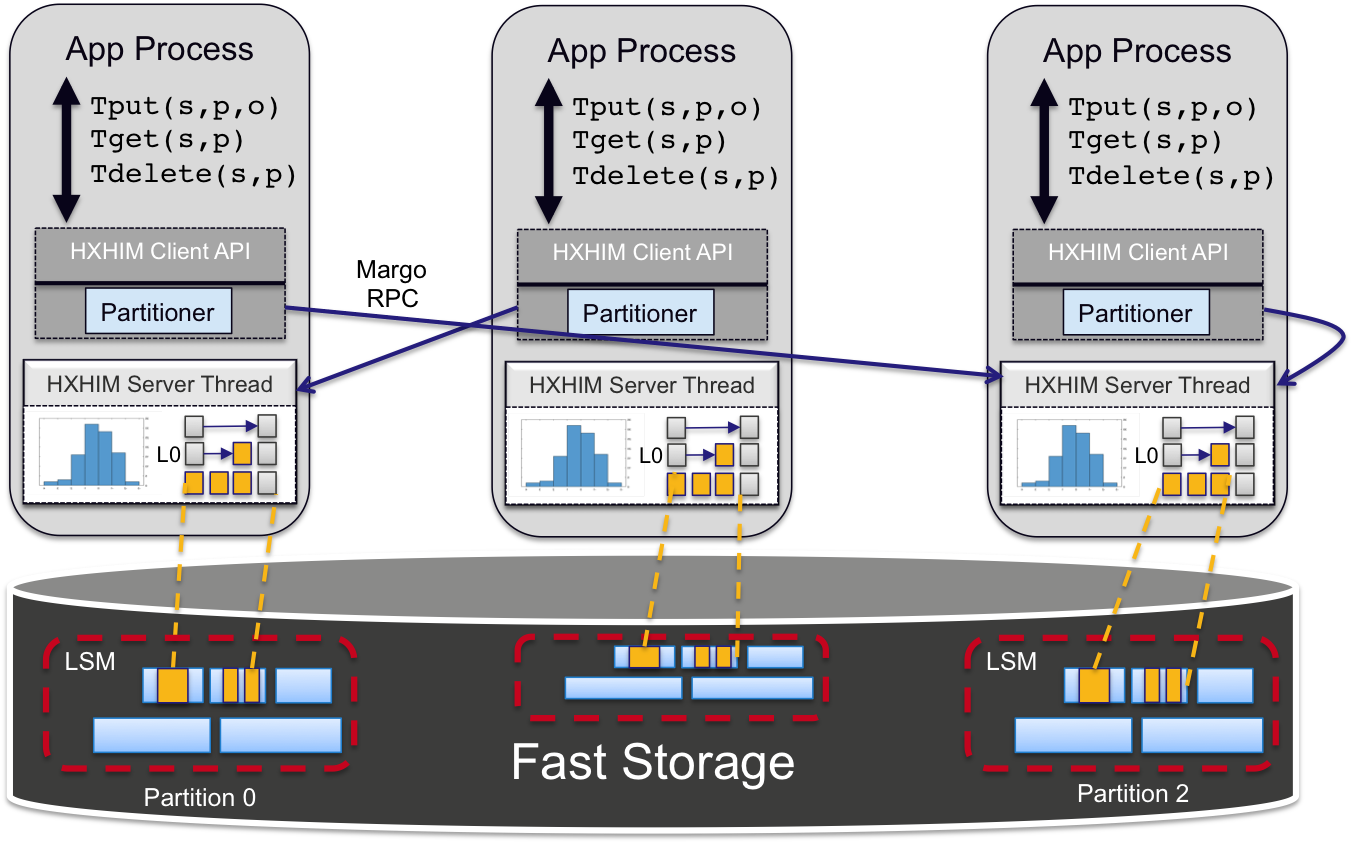
\includegraphics[width=6in]{projects/2.3.6-NNSA/2.3.6.01-LANL-ATDM/hxhim-main}
	\caption{\label{fig:hxhim} Relevant components of the HXHIM
	embeddable service. The client library is provided as a set of API
	calls while the server capability is provided by a thread running
	within the application. Communication uses the Margo and Mercury RPC
	layers to provide efficient support for remote key-value access.}
\end{figure}

Recent progress on HXHIM, a key-value store for HPC platforms, includes the
integration of a new transport layer based on Margo and Mercury (projects
under development by the ECP data libs project). The fundamental architecture
of HXHIM now leverage new support for using a high-performance RPC package
(Mercury) layered beneath a C++ wrapper for Margo (called Thallium). HXHIM
provides bulk (multi-key) primitives that enable efficient use of HPC
interconnects and typical scientific storage workloads.

\begin{figure}[htb]
	\centering
	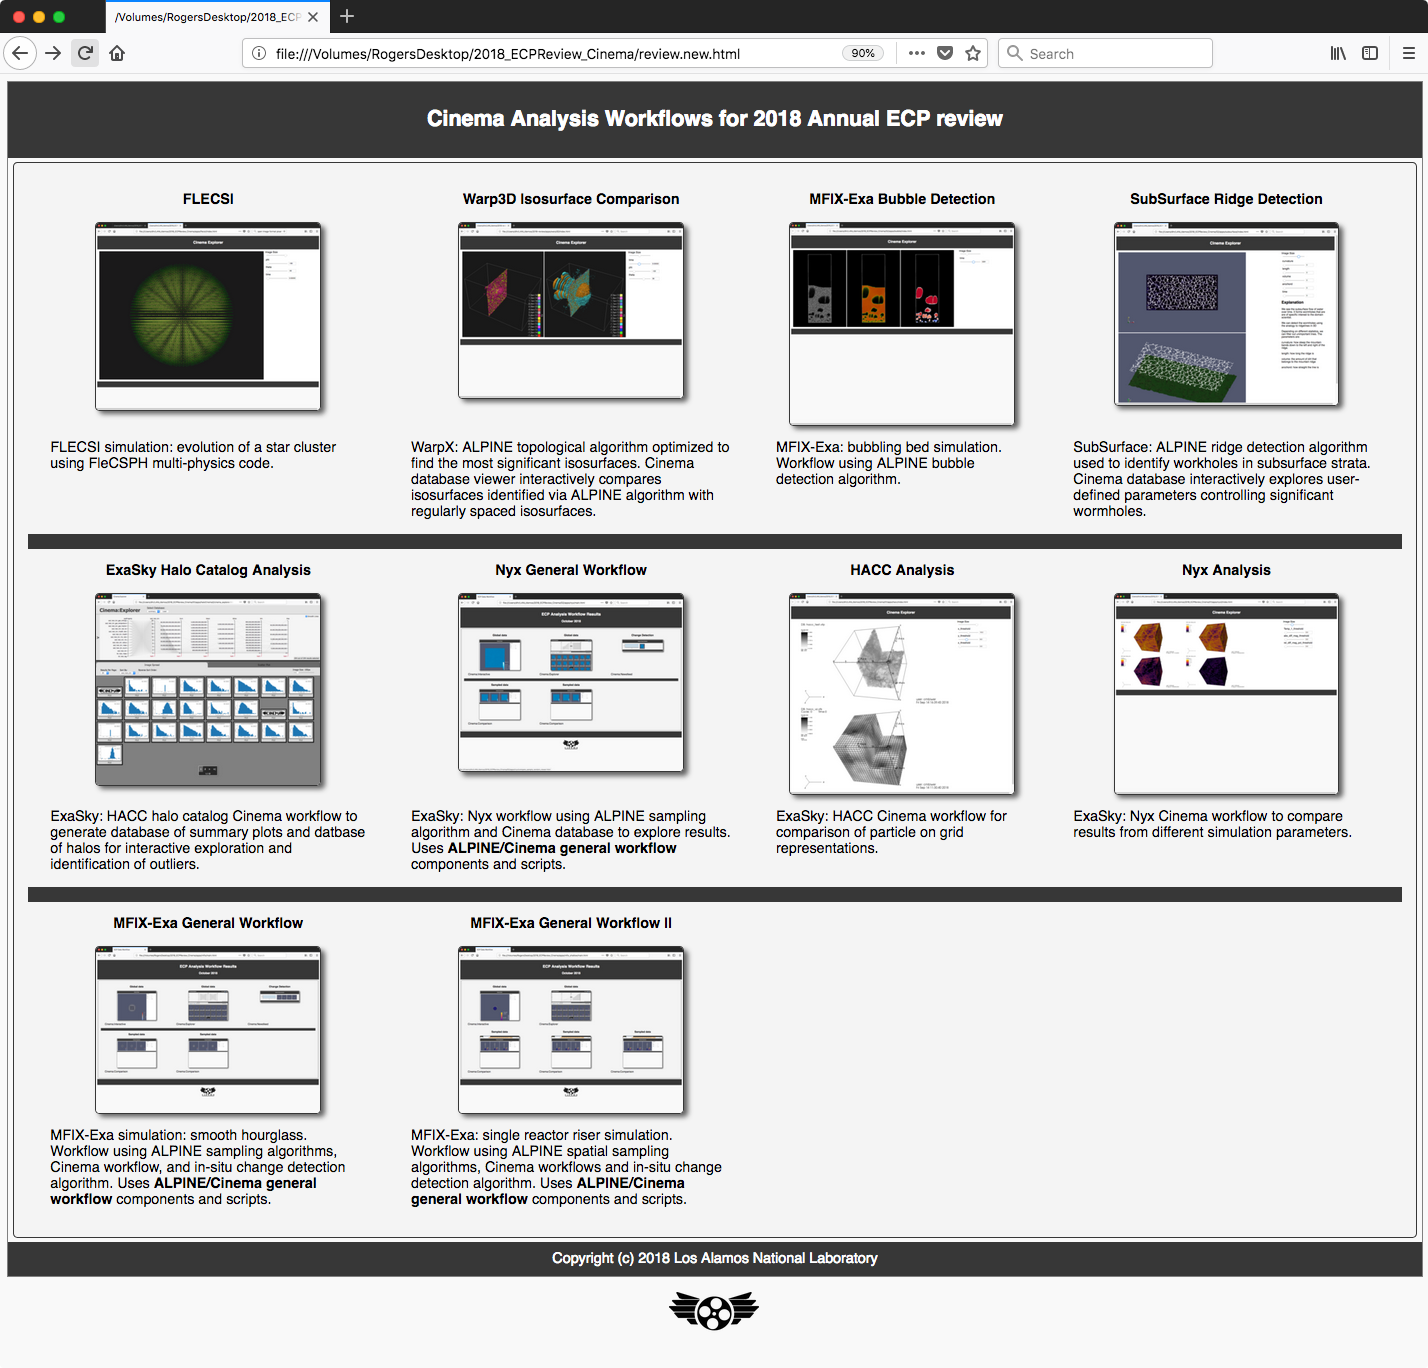
\includegraphics[width=5in]{projects/2.3.6-NNSA/2.3.6.01-LANL-ATDM/ECPReviewScreenshot.png}
	\caption{
        Screen capture of a browser-based set of Cinema viewers 
        for a set of ECP datasets. We ran a variety of ALPINE algorithms
        extracted relevant data features, and then output 
        results as Cinema databases visualized in
        a variety of ways, including comparison views, database
        explorers, and change detection.
    }
\end{figure}

Recent Cinema work has focused on development of capability
and workflows for change detection in-situ data analysis artifacts. These
promote new ways of analyzing ECP data, including
automated and assisted analysis. New capabilities provide 
scientists more options in analyzing and exploring the results of large
simulations by provide a workflow that 1) detects features in-situ, 2)
captures data artifacts in Cinema databases, 3) promotes
post-hoc analysis of the data, and 4)
provides data viewers that allow interactive, structured exploration of the
resulting artifacts. In our most recent milestone, we ran
ALPINE algorithms and Cinema viewer creation workflows on a variety of
ECP and ATDM simulation results to demonstrate integration with applications
and progress in focusing on ECP application needs.
This overall workflow provides a
flexible method of applying new algorithms to the analysis and visualization
of extreme scale data.

\paragraph{Next Steps}
%\textit{Describe what you are working on next.}
Cinema is identifying new application workflows that can be reasonably made
efficient and new analysis methods to apply efficiently for cinema
users.

HXHIM, MarFS, and the monitoring infrastructure have all been descoped
from ECP though the work will continue as part of LANL's Computational Systems
and Software Environments effort. We do not expect this change to alter the
trajectory of any of the descoped projects.
